\documentclass[11pt, oneside]{article}  

\usepackage{style-3yp} %this is the .sty file
\lfoot{James Rhodes} %your name in the footer

\begin{document}
\section{Ammonia Synthesis and Storage}

    \subsection{Cryogenic Distillation Plant Schematic}
    \begin{figure}[ht]
        \centering
        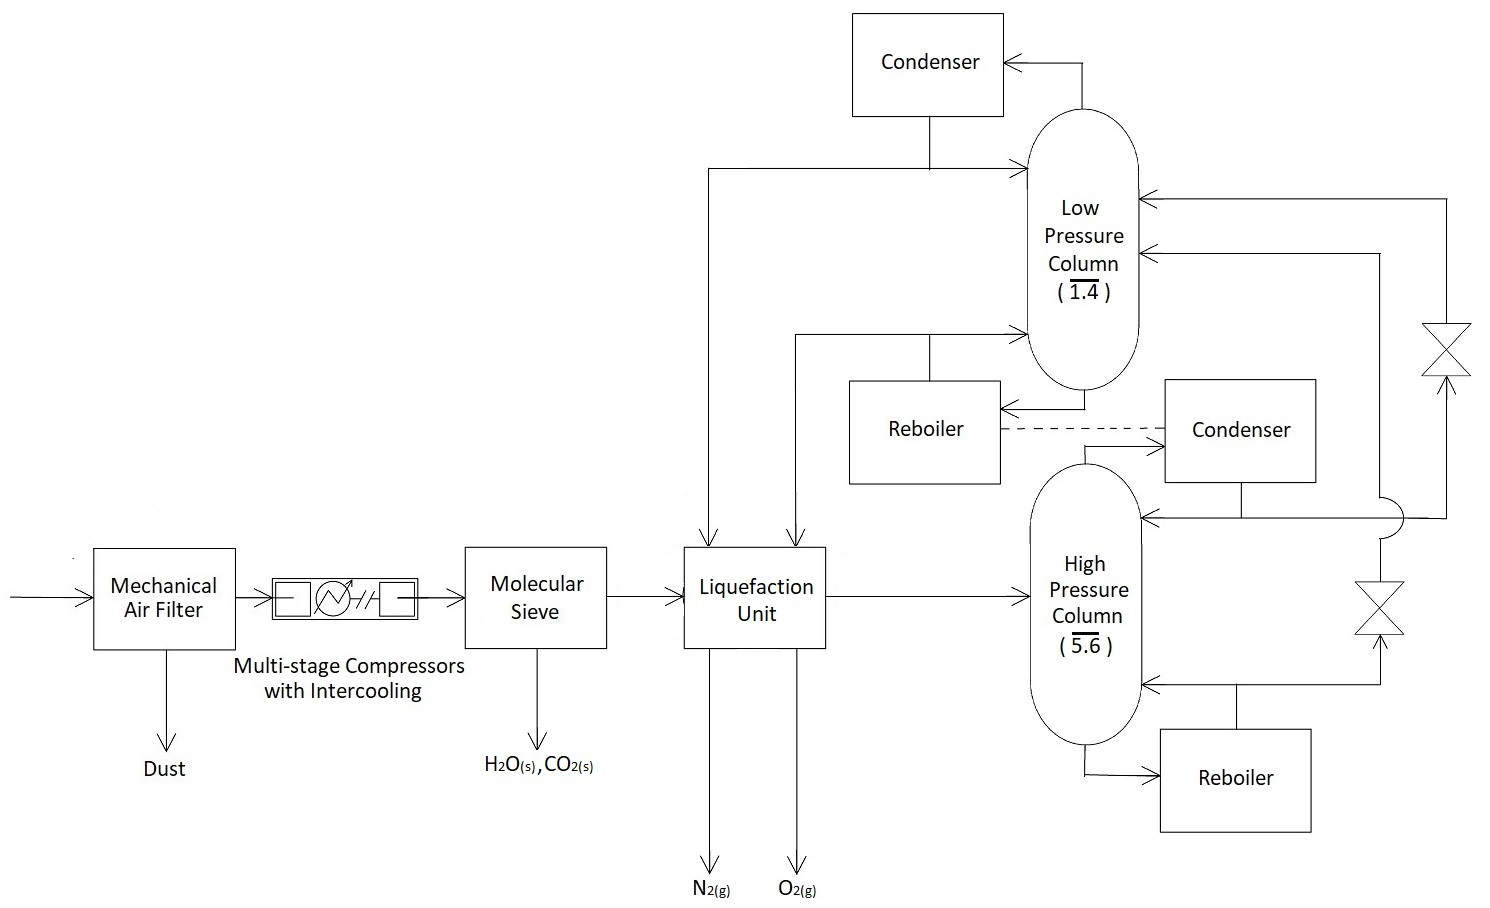
\includegraphics[width=0.87\textwidth]{airseparation/handouts/graphics/plant_diagram.jpg}
        \caption{Cryogenic Distillation Plant Schematic (adopted from Linde Engineering) [Slide 7]}
        \label{fig:plant_schematic}
    \end{figure}
    
    \subsection{Liquefaction Unit}
    \begin{figure}[ht]
        \centering
        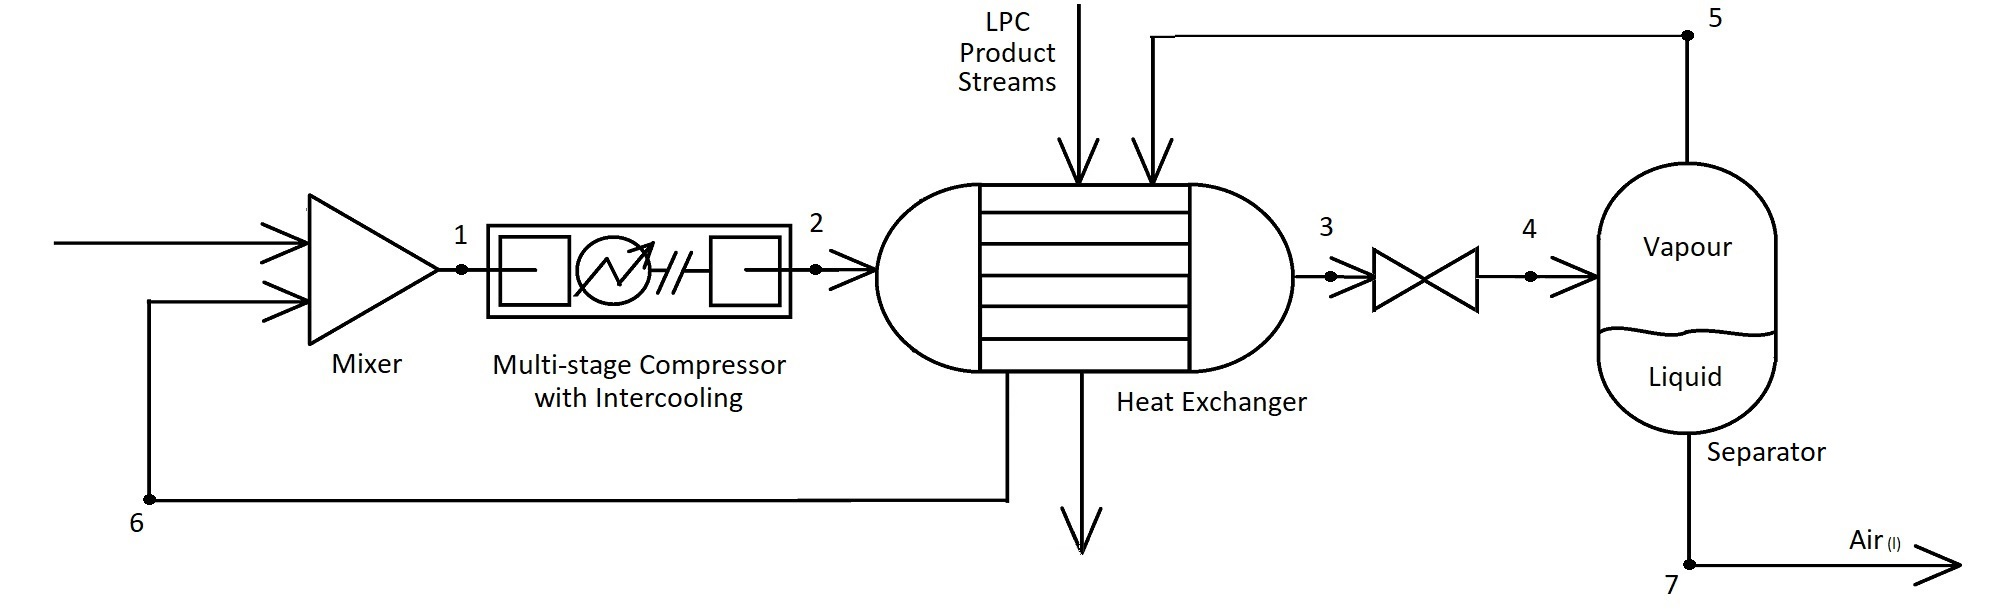
\includegraphics[width=1.1\textwidth]{airseparation/handouts/graphics/labelled_liquefier_diagram.jpg}
        \caption{Modified Linde-Hampson Liquefaction Cycle [Slide 8]}
        \label{fig:liquefier}
    \end{figure}
    
    \newpage
    
    \subsection{Double Distillation Column System}
    \begin{figure}[ht]
        \centering
        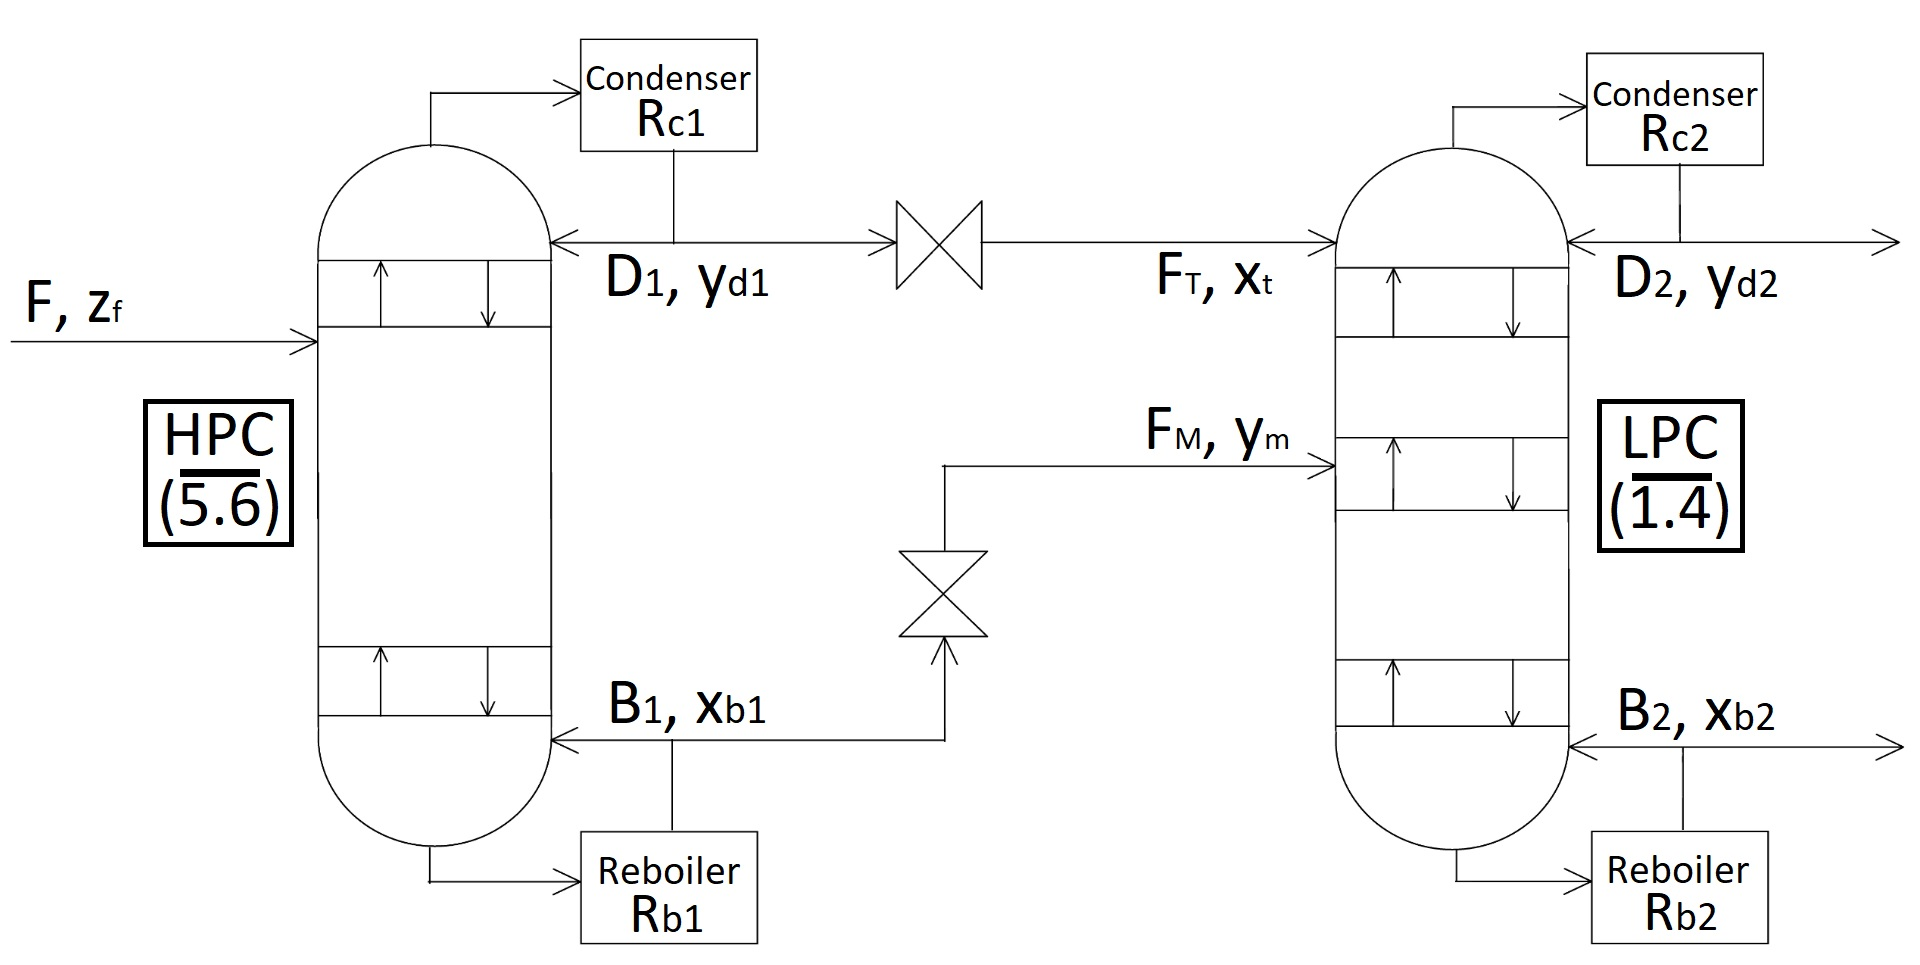
\includegraphics[width=0.9\linewidth]{airseparation/handouts/graphics/labelled_columns_diagram_simple.jpg}
        \caption{Diagram of High and Low Pressure Column [Slide 10]}
        \label{fig:column_linkage}
    \end{figure}
    \hfill
    \hfill
    \begin{figure}[ht]
        \begin{subfigure}{0.49\textwidth}
            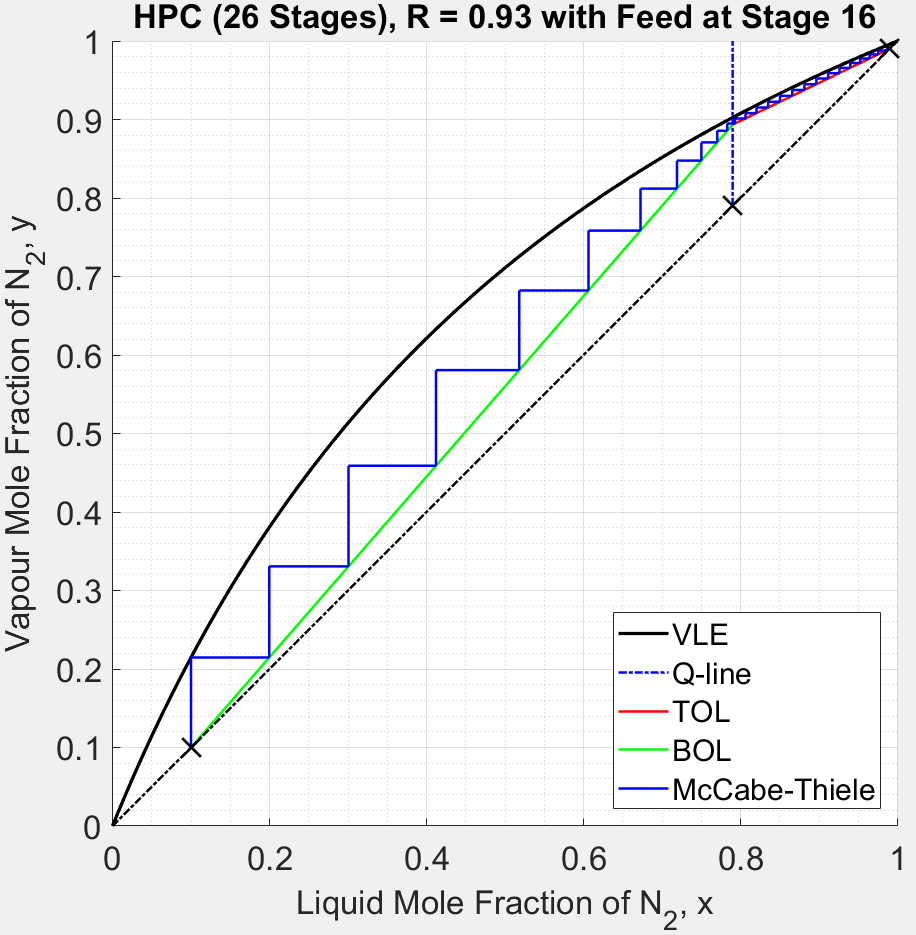
\includegraphics[width=\linewidth]{airseparation/handouts/graphics/HPC_v0a.jpg}
            \caption{High Pressure Column}
            \label{fig:HPC_v0}
        \end{subfigure}
        \hspace*{\fill} % separation between the subfigures
        \begin{subfigure}{0.49\textwidth}
            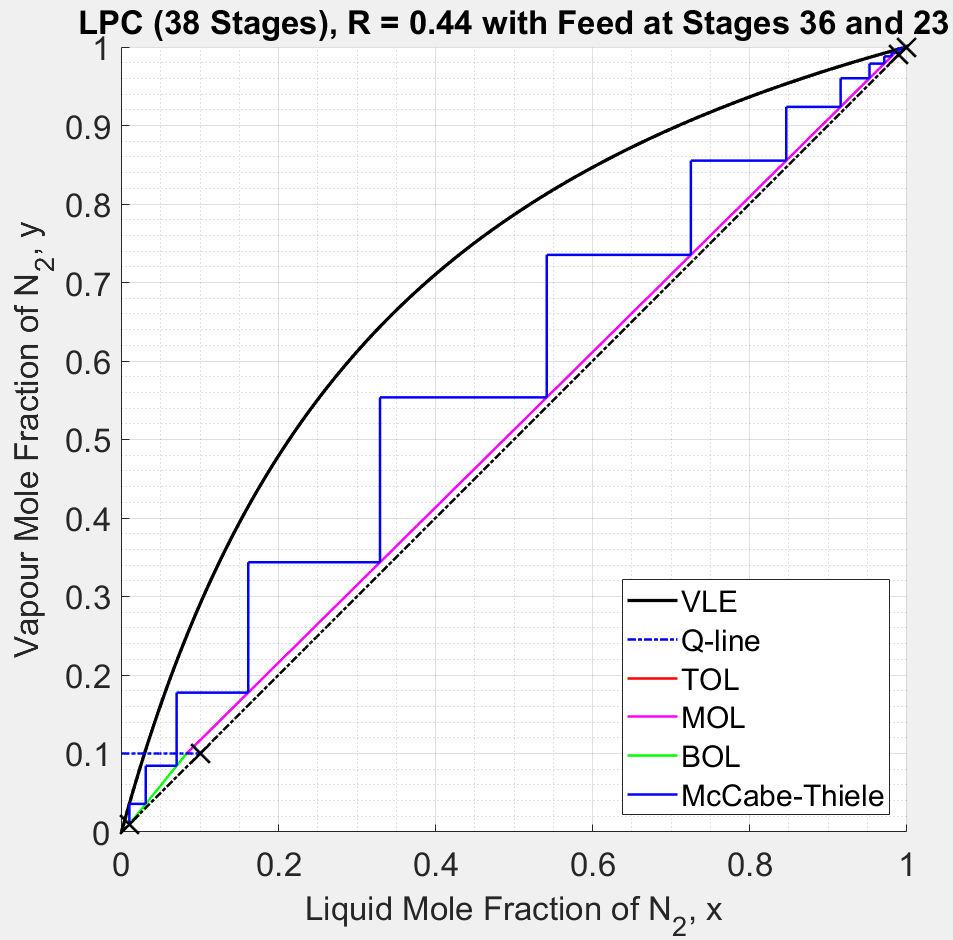
\includegraphics[width=\linewidth]{airseparation/handouts/graphics/LPC_v0a.jpg}
            \caption{Low Pressure Column}
            \label{fig:LPC_v0}
        \end{subfigure}
        \caption{McCabe-Thiele Construction of Initial Model [Slide 11]}
        \label{fig:mccabe_v0}
    \end{figure}
    
    \begin{figure}[ht]
        \begin{subfigure}{0.49\textwidth}
            \centering
            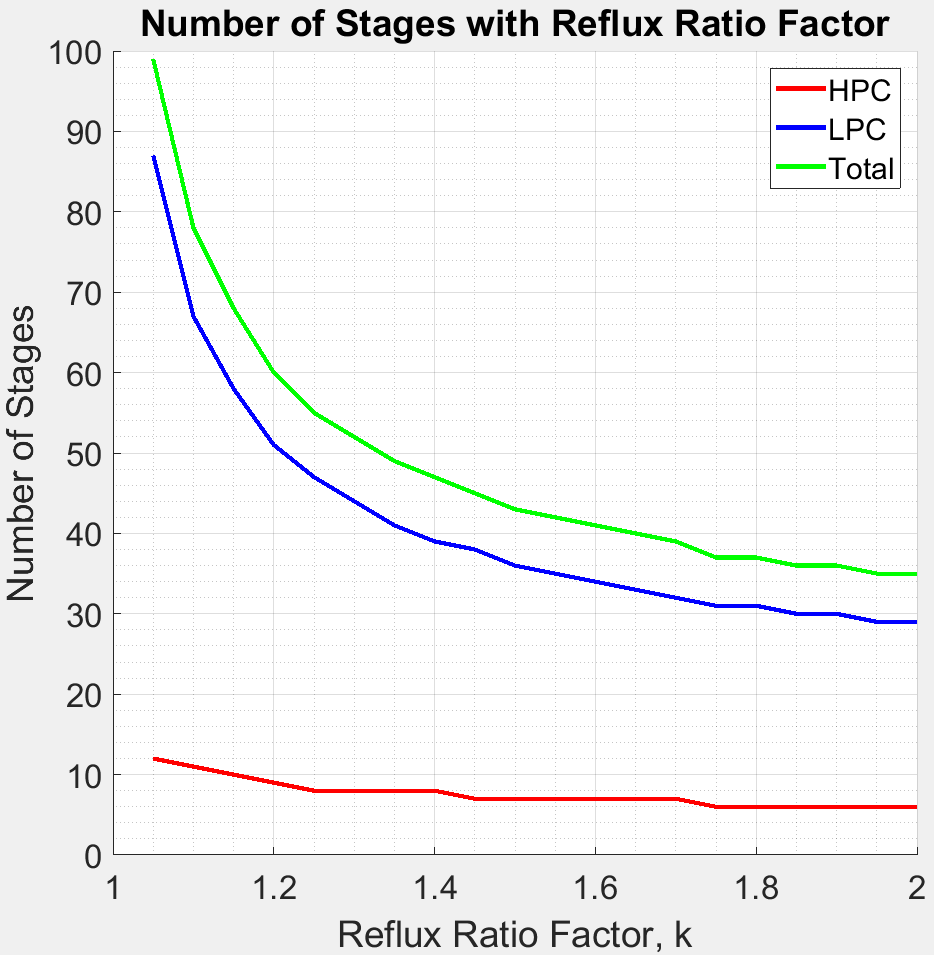
\includegraphics[width=\linewidth]{airseparation/handouts/graphics/graph-stages_vs_R_va.jpeg}
            \caption{Number of Equilibrium Stages against \newline Reflux Ratio Factor}
            \label{fig:stage_vs_R}
        \end{subfigure}
        \hspace*{\fill} % separation between the subfigures
        \begin{subfigure}{0.49\textwidth}
            \centering
            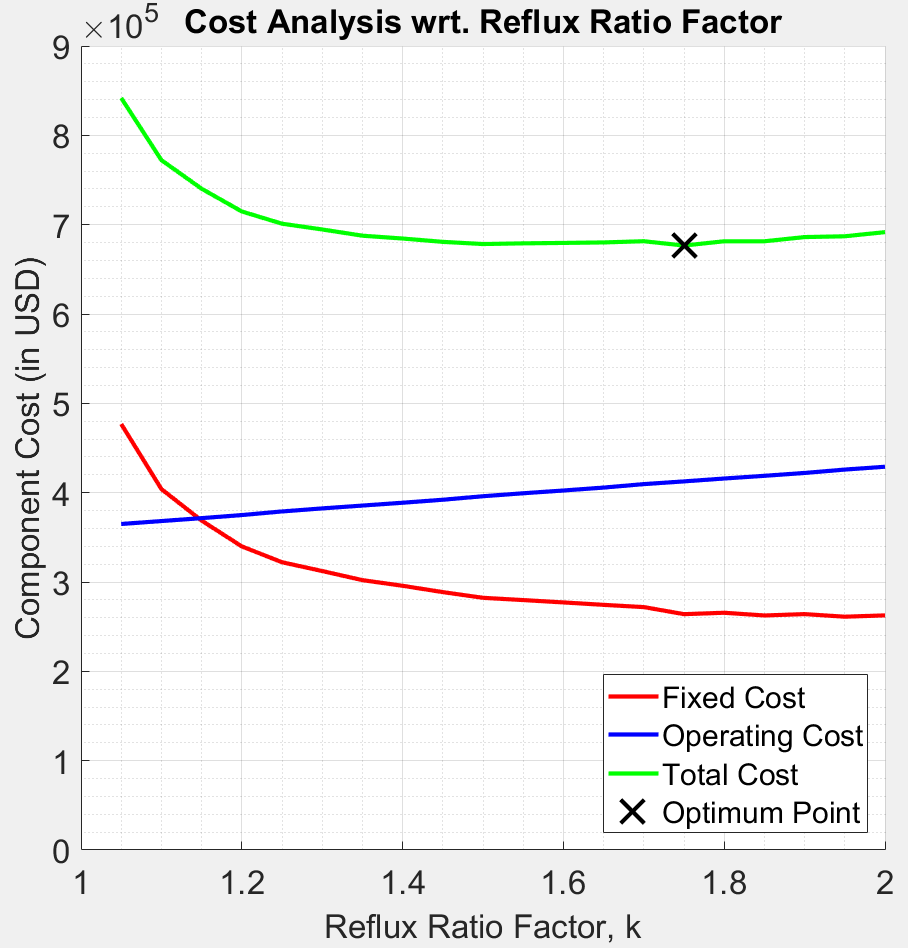
\includegraphics[width=\linewidth]{airseparation/handouts/graphics/column_cost_vs_reflux_va.jpeg}
            \caption{Column Cost Analysis \newline $_$ }
            \label{fig:cost_vs_R}
        \end{subfigure}
        \caption{Column Optimisation and Cost Analysis [Slide 12-13]}
        \label{fig:cost_analysis}
    \end{figure}
    
    \begin{figure}[ht]
        \begin{subfigure}{0.49\textwidth}
            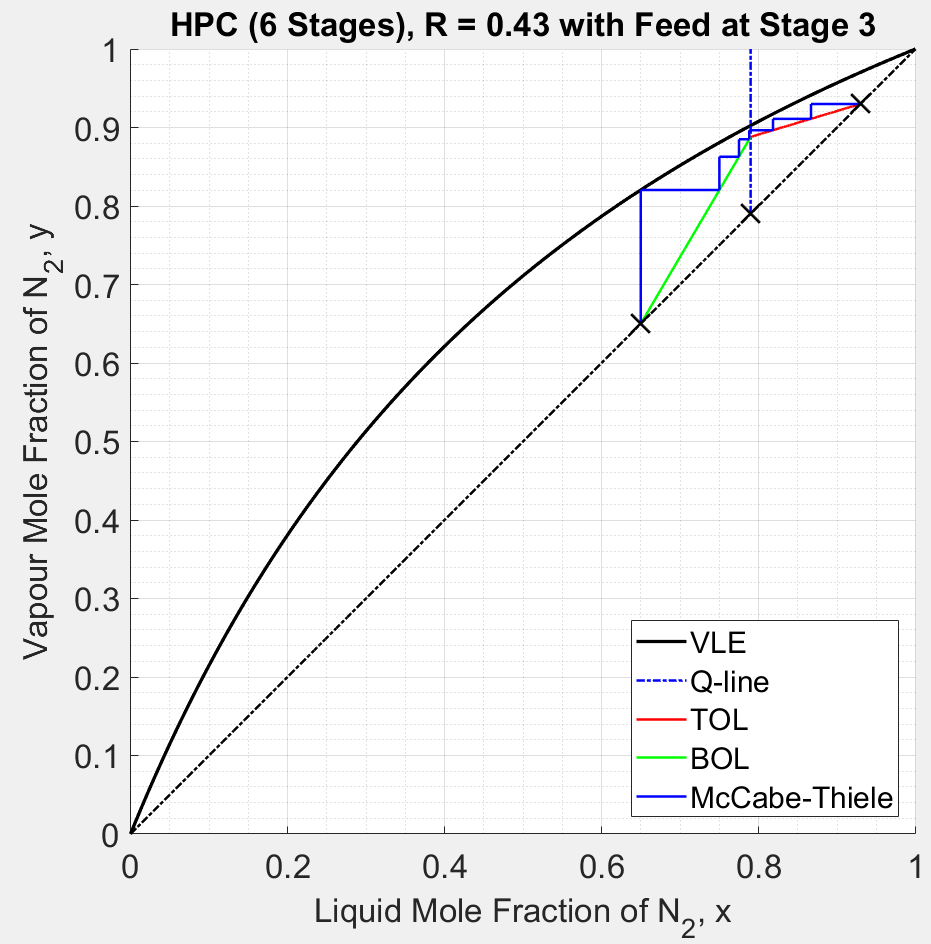
\includegraphics[width=\linewidth]{airseparation/handouts/graphics/HPC_v1a.jpeg}
            \caption{High Pressure Column}
            \label{fig:HPC_v1}
        \end{subfigure}
        \hspace*{\fill} % separation between the subfigures
        \begin{subfigure}{0.49\textwidth}
            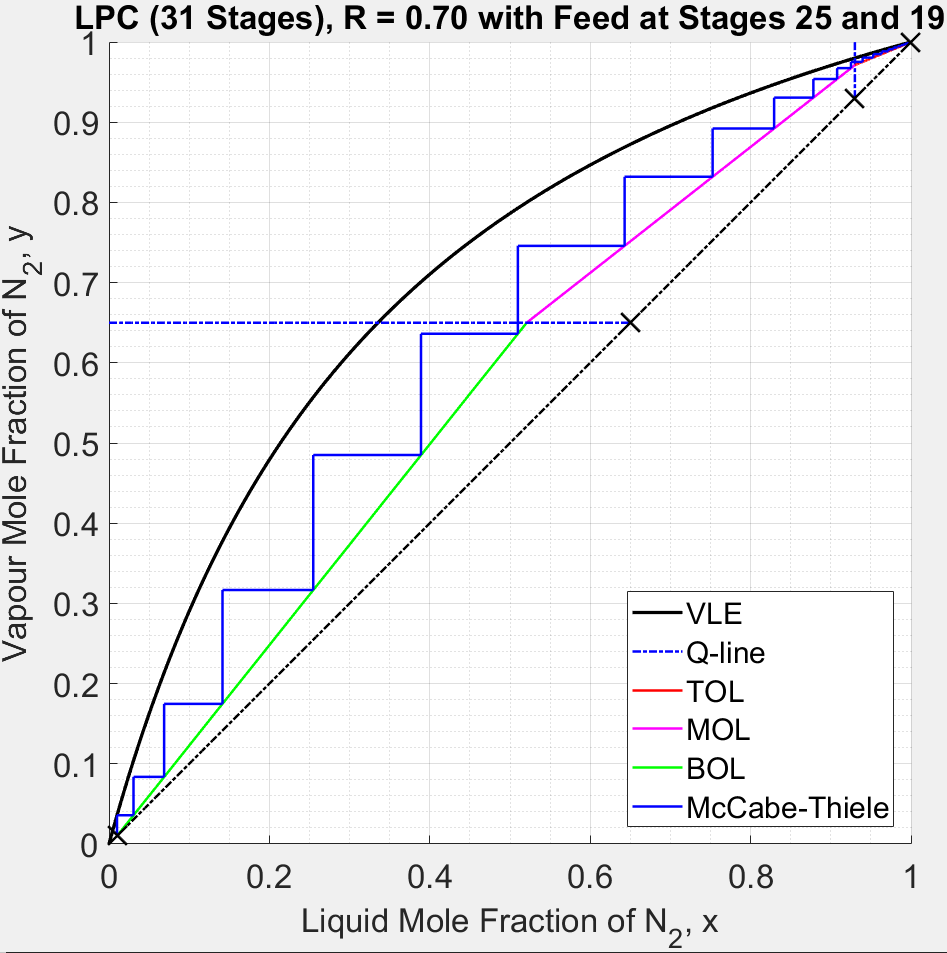
\includegraphics[width=\linewidth]{airseparation/handouts/graphics/LPC_v1a.jpeg}
            \caption{Low Pressure Column}
            \label{fig:LPC_v1}
        \end{subfigure}
        \caption{McCabe-Thiele Construction of Final Model [Slide 14]}
        \label{fig:mccabe_v1}
    \end{figure}
    
\end{document}